\section{Research} \label{questions}
In this section the research questions for the thesis are formulated. What is research method will be used and how the questions are being validated.

\subsection{Context}
What is the context of the research. 

\subsection{Research questions}

How can model diff help testers finding bugs???
%% specify: "What form of the answer
%% remove ambiguity
%% specify: which factors influences the RQ

- How are changes in state models detected? -> Fernando the video. no paper in TESTAR, Murphy. Image recognition might help in telling difference. 

Could it be possible to use abstract image recognition. make a screenshot of an SUT and then fill in parts, like a Text box as a rectangle, button as a solid block etc. 

% 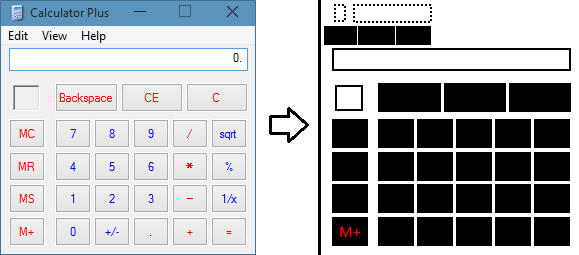
\includegraphics{document/pics/abstract-ui.png}

- What can TESTAR learn from Murphy?

- What other tools are available that uses state model difference to reason about a change? 

- How can difference in the state model become visible inside build-in state model visualisation?

- How does the build-in state model work?

sub question: How to get a useful model for the model diff.
what is a useful model... -> depends on model diff requirements

sub question- How can we tell TESTAR to ignore complete entire widgets for state abstraction?

% discusion points:
%- How can developers of GUI help in creating better models generated by TESTAR?
%- Is it bad to add testing hooks into an application? I hypothesise that adding hooks into code is not bad and can be considered a good practice when creating unit or even integration tests. Is my hypothesis correct and is it a correct hypothesis for GUI testing? I know that Microsoft provides attached properties for XAML based application (AutomationIds). Those properties are then used in code-based GUI testing.

\subsection{Research method}

\subsection{Validity}

\subsection{Planning}